\documentclass{article}

\usepackage[margin=1in]{geometry}

\usepackage{amsmath}
\usepackage{amssymb}
\usepackage{calc}
\usepackage{caption}
\usepackage{graphicx}
\usepackage{indentfirst}
\usepackage{lmodern}
\usepackage{newfloat}
\usepackage[dvipsnames]{xcolor}
\usepackage{tikz, tikz-qtree}
\usepackage[utf8]{inputenc}
\usepackage[T1]{fontenc}
\usepackage[normalem]{ulem}
\usepackage[hidelinks]{hyperref}


\setlength{\parskip}{5pt}%

\DeclareFloatingEnvironment[fileext=lod]{diagram}
\captionsetup[diagram]{labelformat=empty}
\captionsetup[figure]{labelformat=empty}

\usetikzlibrary{trees}
\usetikzlibrary{positioning}
\tikzset{level distance=45pt}
\tikzset{
  edge from parent/.style= { draw, edge from parent path= {
      (\tikzparentnode.south)
      -- +(0,-15pt)
      -| (\tikzchildnode)
    }
  }
}


\begin{document}

\begin{titlepage}
  \centering
  
  \vfill{
    \bfseries\Huge
    Universidade Federal de Minas Gerais\\[5pt]
    \bfseries\Large
    Bacharel em Sistemas de Informação \\
    Algoritmos e Estruturas de Dados 3\\
  }
  
  \vfill
  
  
\includegraphics[width=13cm]{images/ufmg_logo.jpg}
  
  \vfill{
    \bfseries\Large
    Trabalho Prático 1\\
    Agosto 2017\\
  }
  \vfill{
    \bfseries\large
    Gabriel Silva Bastos\\[5pt]
    Matrícula: 2016058204
  }
\end{titlepage}


\section{Introdução}
Nubby está de volta, desta vez para organizar um campeonato de \textit{Mortal Kontest}. Participarão $\{ v_1, \hdots, v_n \}$ amigos $(1 \leq n \leq 25)$, e Nubby ficará encarregado apenas da organização de todas as $n - 1$ rodadas. Em cada rodada, dois amigos dos que não foram eliminados serão escolhidos aleatóriamente para o embate, e o que perder é eliminado do campeonato. Desta forma, a última rodada será entre os dois amigos restantes, e o vencedor desta é o grande campeão.

Nubby possui dados de batalhas anteriores entre seus amigos, e através destes calculou a probabilidade de cada amigo vencer os demais em um embate. Através destas probabilidades, Nubby quer calcular a probabilidade de cada um de seus amigos vencer o campeonato.


\section{Visão Geral da Solução}
A entrada consiste de um número $n$ de jogadores, e uma matriz $V \in \mathbb{M}_{n \times n}$ contendo as probabilidades calculadas por Nubby. A posição $i, j$ na matriz contém a probabilidade $V_{i,j} \in [0,1]$ do jogador $v_i$ vencer o jogador $v_j$ em um embate. Além disso, todas posições da forma $i, i$ contém o valor $0$, que é a probabilidade de um jogador vencer à si mesmo, e as demais posições $i, j$ satisfazem $V_{i,j} = 1 - V_{j,i}$.
\[
  \begin{bmatrix}
      0 & \hdots  & V_{1,n} \\
      \vdots & \ddots  & \vdots \\
      V_{n,1} & \hdots & 0
  \end{bmatrix}
\]
Para ilustrar a solução, utilizaremos um caso particular onde $n = 3$. A seguinte árvore representa os possíveis desdobramentos do campeonato neste caso:
\begin{diagram}[h]
  \centering
  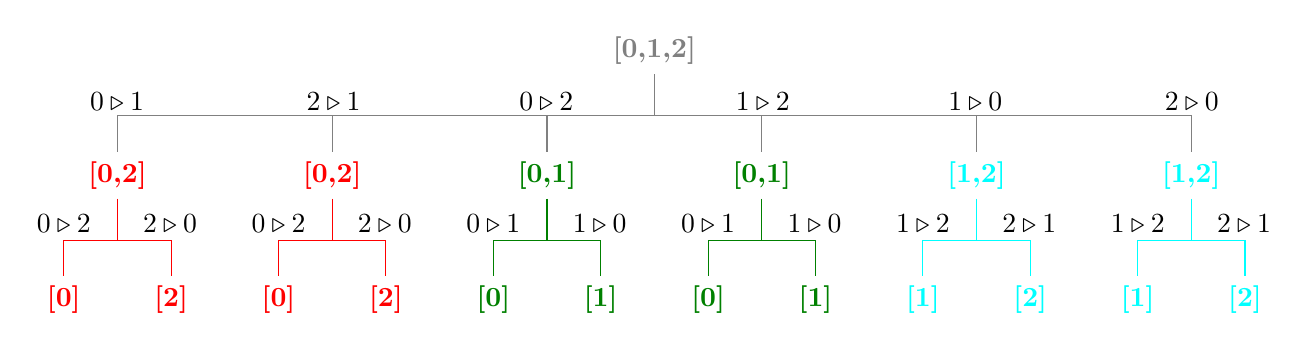
\begin{tikzpicture}[sibling distance=20pt]
    \tikzset{every tree node/.style={font=\bf}}
    \Tree [
      .\node[text=gray] (root) {[0,1,2]};
          \edge[draw=gray]; [.\node[text=Red] (s1) {[0,2]}; \edge[draw=Red]; {\color{Red} [0]}
                                                            \edge[draw=Red]; {\color{Red} [2]} ]
          \edge[draw=gray]; [.\node[text=Red] (s2) {[0,2]}; \edge[draw=Red]; {\color{Red} [0]}
                                                            \edge[draw=Red]; {\color{Red} [2]} ]
          %
          \edge[draw=gray]; [.\node[text=Green] (s3) {[0,1]}; \edge[draw=Green]; {\color{Green} [0]}
                                                              \edge[draw=Green]; {\color{Green} [1]} ]
          \edge[draw=gray]; [.\node[text=Green] (s4) {[0,1]}; \edge[draw=Green]; {\color{Green} [0]}
                                                              \edge[draw=Green]; {\color{Green} [1]} ]
          %
          \edge[draw=gray]; [.\node[text=Cyan] (s5) {[1,2]}; \edge[draw=Cyan]; {\color{Cyan} [1]}
                                                             \edge[draw=Cyan]; {\color{Cyan} [2]} ]
          \edge[draw=gray]; [.\node[text=Cyan] (s6) {[1,2]}; \edge[draw=Cyan]; {\color{Cyan} [1]}
                                                             \edge[draw=Cyan]; {\color{Cyan} [2]} ]
    ]
    
    \node [below left=.15cm of root, xshift=-5.6cm] {$0 \triangleright 1$};
    \node [below left=.15cm of root, xshift=-2.85cm] {$2 \triangleright 1$};
    \node [below left=.15cm of root, xshift=-0.15cm] {$0 \triangleright 2$};
    \node [below left=.15cm of root, xshift=2.6cm] {$1 \triangleright 2$};
    \node [below left=.15cm of root, xshift=5.3cm] {$1 \triangleright 0$};
    \node [below left=.15cm of root, xshift=8.05cm] {$2 \triangleright 0$};

    \node [below left=.1cm of s1, xshift=.35cm] {$0 \triangleright 2$};
    \node [below left=.1cm of s1, xshift=1.7cm] {$2 \triangleright 0$};
    
    \node [below left=.1cm of s2, xshift=.35cm] {$0 \triangleright 2$};
    \node [below left=.1cm of s2, xshift=1.7cm] {$2 \triangleright 0$};
    
    \node [below left=.1cm of s3, xshift=.35cm] {$0 \triangleright 1$};
    \node [below left=.1cm of s3, xshift=1.7cm] {$1 \triangleright 0$};
    
    \node [below left=.1cm of s4, xshift=.35cm] {$0 \triangleright 1$};
    \node [below left=.1cm of s4, xshift=1.7cm] {$1 \triangleright 0$};
    
    \node [below left=.1cm of s5, xshift=.35cm] {$1 \triangleright 2$};
    \node [below left=.1cm of s5, xshift=1.7cm] {$2 \triangleright 1$};
    
    \node [below left=.1cm of s6, xshift=.35cm] {$1 \triangleright 2$};
    \node [below left=.1cm of s6, xshift=1.7cm] {$2 \triangleright 1$};
  \end{tikzpicture}
\end{diagram}\\
Cada nó da árvore corresponde ao grupo $G$ ainda presente no campeonato.

\noindent As folhas contém grupos unitários, que indicam o campeão do desdobramento descrito pelo caminho da raiz até a folha.

\noindent O rótulo $i \triangleright j$ para cada aresta indica que na rodada e configuração correspondentes os jogadores $i$ e $j$ foram escolhidos para o embate, e o jogador $i$ venceu.

\noindent Cada nível de arestas corresponde à uma rodada, e cada aresta é uma possibilidade para a rodada. Em cada nível, o número $a$ de arestas é
\[ a = \binom{|G|}{2} = \frac{{|G|}^2 - |G|}{2} \]

\pagebreak

\noindent Cada caminho da raiz até um nó na árvore descreve um desdobramento do campeonato, e portanto possui uma probabilidade associada para cada possível vencedor. Tais probabilidades são compostas pela combinação de dois itens:
\begin{itemize}
  \item A probabilidade associada à rodada: Cada rodada é modelada como uma aresta para cada escolha de um vencedor e um perdedor possível. Cada aresta corresponde à equiprovável da escolha dos jogadores vezes a chance do vencedor vencer.
    \[ P(i \triangleright j) = \frac{1}{a} \cdot V_{i,j} = \frac{2}{{|G|}^2 - |G|} \cdot V_{i,j} \]
  \item A probabilidade associada à subárvore conectada pela aresta, que corresponde à combinação das probabilidades das subarestas.
\end{itemize}

\noindent O segundo item denota um subproblema, pois a subárvore conectada por cada aresta pode ser considerada um subcampeonato. Como é notável no diagrama, vários subcampeonatos equivalentes ocorrem quando geramos a árvore de desdobramentos. Estes foram dispostos com a mesma cor para melhor visualização.

\noindent Efetivamente, a probabilidade de um jogador vencer o campeonato é o somatório das probabilidades dos desdobramentos em que ele vence.

\subsection{Estratégia de Memorização}
Os subproblemas foram definidos como os subcampeonatos. Um subcampeonato é constituido pela exclusão de alguns membros do campeonato original $C$, devido à eliminação das rodadas passadas. Portanto, todos subcampeonatos possíveis pertencem ao conjunto potência de $C$.

Como todos os desdobramentos do campeonato $C$ são necessários para a solução do problema, gerar o conjunto potência se torna necessário. Porém, os subcampeonatos com menos de 2 jogadores não são interessantes, então podemos excluí-los da memorização. Portanto, é necessário memorizar $m$ grupos
\begin{align*}
  m & = |\mathcal{P}(C)| - |C| - 1 \\
  & = 2^n - n - 1
\end{align*}
Para memorizar tais grupos, um vetor foi adotado. Também foi necessária uma forma eficiente de identificar cada grupo no vetor. Considerando que o tamanho máximo de jogadores definido por Nubby foi $25$, um inteiro de largura fixa de 32 bits é utilizado para identificar cada grupo. Cada bit no corresponde à presença do jogador no grupo
\begin{align*}
  0 \hdots 0 \> 00011010_b &\equiv [1, 3, 4] \\
  0 \hdots 1 \> 00100101_b &\equiv [0, 2, 5, 8] \\
  0 \hdots 0 \> 11111111_b &\equiv [0, 1, 2, 3, 4, 5, 6, 7]
\end{align*}
Para converter desta representação para um índice no vetor, é necessário descontar os grupos unitários e o grupo vazio que não foram considerados. A seguinte função realiza esta compensação em um identificador de grupo $g$:
\[ \varphi(g) = g - \lceil \log_2 g \rceil - 1 \]


\pagebreak


\section{Análise de Complexidade}

\subsection{Espacial}
\noindent Para a matriz $M$, são alocados $n^2$ \textit{floats}.\\[5pt]
Para cada subgrupo, são alocados $n$ \textit{floats}, correspondendo à probabilidade de cada jogador vencer.\\
Aos jogadores não presentes no grupo é atribuida probabilidade $0$ de vencer. \\[5pt]
São $2^n - n - 1$ grupos, portanto $(2^n - n - 1) \cdot n$ \textit{floats} alocados. \\[5pt]
A complexidade espacial final é
\begin{align*}
  & \Theta \left( n^2 + (2^n - n - 1) \cdot n \right) \\
  & \Theta \left( n^2 + n \cdot 2^n - n^2 - n \right) \\
  & \Theta \left(n \cdot 2^n - n \right) \\
  & \Theta \left(n \cdot 2^n \right)
\end{align*}

\subsection{Temporal}
Portanto, a complexidade é $\mathcal{O}(\log n)$.


\section{Análise Experimental}
A análise experimental da implementação é mostrada pela figura 1. Para realizar os experimentos, foi feito um gerador de entradas. Para um valor $n$, é gerada uma entrada contendo um vetor de tamanho $n$, e $n / 2$ operações de busca e atualização intercaladas. O intervalo em cada operação é aleatório, mas a largura do intervalo é fixa em $n / 3$. Para medir o tempo de execução do código, foi utilizada a informação de uso de recursos fornecida pelo sistema operacional linux. Os valores $n$ foram escolhidos estrategicamente para cada teste. A razão inicial é verificar, de forma geral, o comportamento dos algoritmos para casos genéricos.
\vspace{-10pt}
\begin{figure}[h]
  \centering
  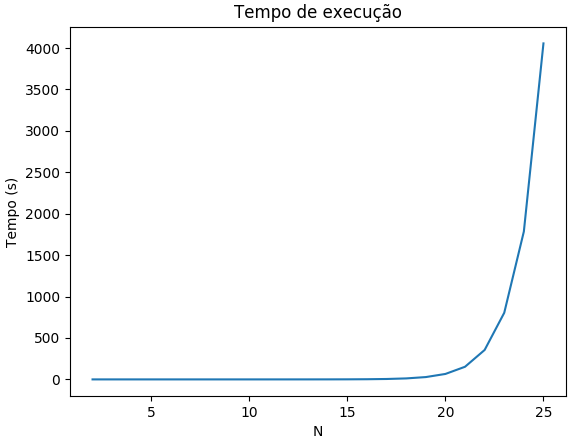
\includegraphics[width=0.49\linewidth]{images/time.png}
  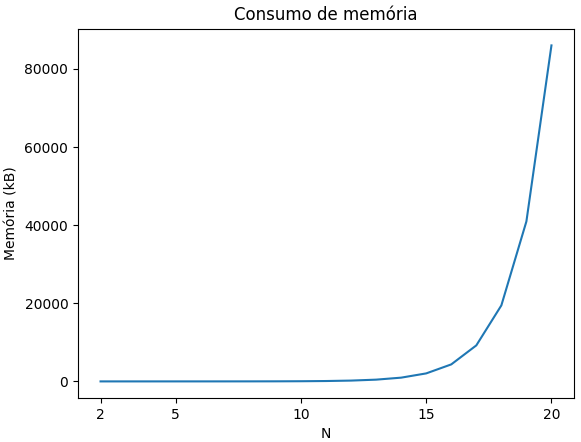
\includegraphics[width=0.49\linewidth]{images/space.png}
  \caption{Figura 1: Teste experimental}
\end{figure}\\
Nos gráficos da figura 1 é notável o ganho em eficiência da árvore de segmentos sobre a matriz.

\pagebreak

\section{Conclusão}
O objetivo do trabalho foi atingido ao demonstrar as diferenças na eficiência das soluções propostas, tanto teoricamente quanto experimentalmente. Tornou-se evidente o grande ganho obtido na performance ao se utilizar uma estruturação de dados adequada.



\end{document}
